% Kap. 3 -- Neuaufbau 2026-11-05, Stil "luftig" 2026-11-06 (Backup: ../elektronik-1_backup_2026-11-05)
% Quellen: alter Kap. 3, Praktikum P2 (Opamp-Oszillator), MSP HS14/15/17/19/22 (keine Folien Kap. 3 gefunden)
\section{Komparator, Schmitt-Trigger, Oszillator}\label{sec:komparator}

\subsection{Komparator}

\begin{minipage}[c]{0.3\columnwidth}
	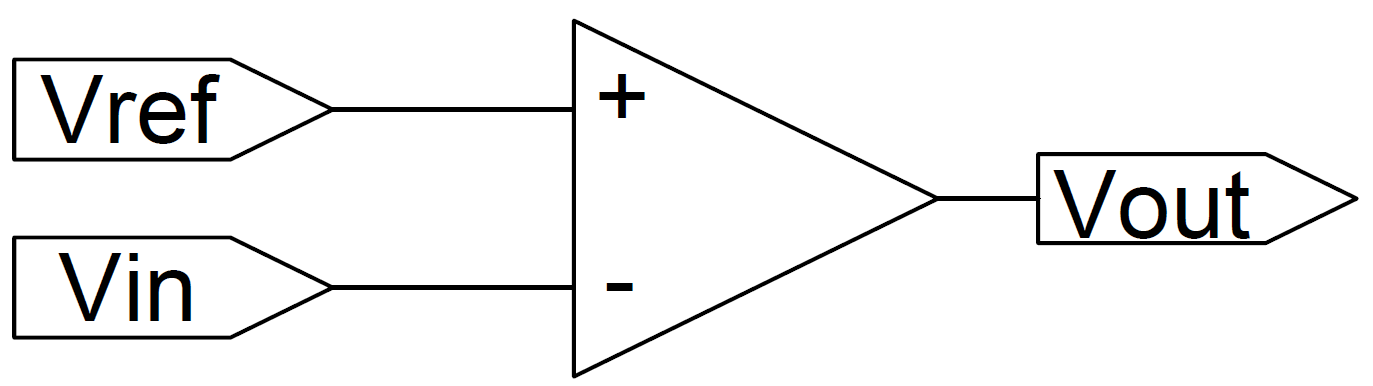
\includegraphics[width=\columnwidth]{images/komparator.png}
\end{minipage}
\hfill
\begin{minipage}[c]{0.3\columnwidth}
	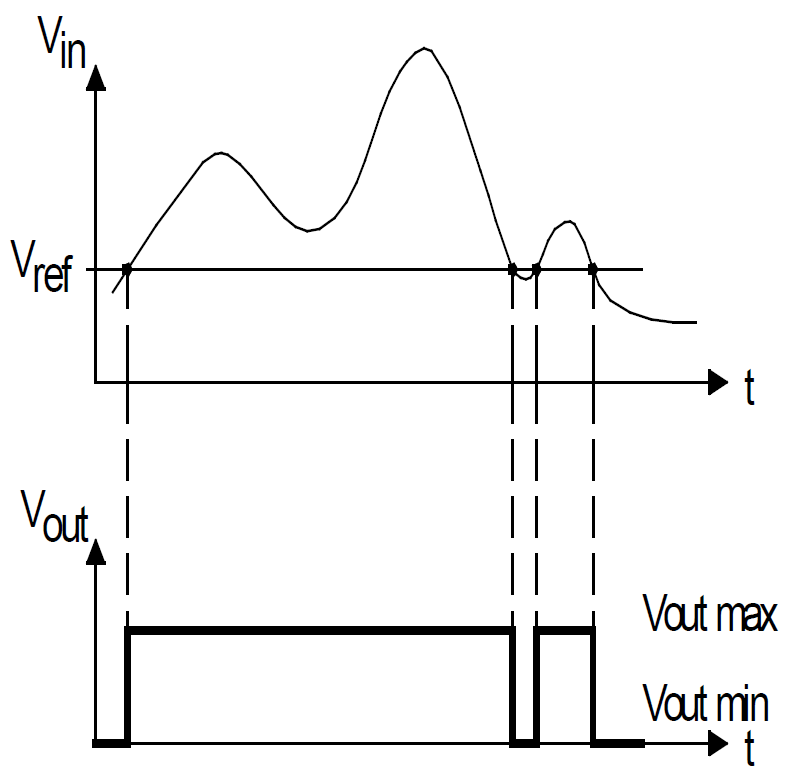
\includegraphics[width=\columnwidth]{images/signalverlauf_komparator.png}
\end{minipage}
\hfill
\begin{minipage}[c]{0.36\columnwidth}
	OpAmp \textbf{ohne Gegenkopplung} \textrightarrow\ Ausgang am Anschlag: \\
	$V_{\rm opp} > V_{\rm opn}$ \textrightarrow\ $V_{\rm out,max}$ \\
	sonst $V_{\rm out,min}$ \\
	Rauschen \textrightarrow\ Glitches
\end{minipage}

\vspace{4pt}
{\renewcommand{\arraystretch}{1.45}
\begin{tabularx}{\columnwidth}{@{}l X@{}}
	\toprule
	\textbf{Komparator-IC}     & schnell (keine Sättigung, grosse Slew-Rate); \textbf{nicht} mit Gegenkopplung (instabil) \\
	\textbf{OpAmp als Komparator} & sättigt im Anschlag \textrightarrow\ schaltet verzögert \textrightarrow\ Oszillator bei hohen $f$ langsamer \\ \bottomrule
\end{tabularx}}

\subsection{Schmitt-Trigger}\label{sec:schmitt}

\begin{minipage}[c]{0.36\columnwidth}
	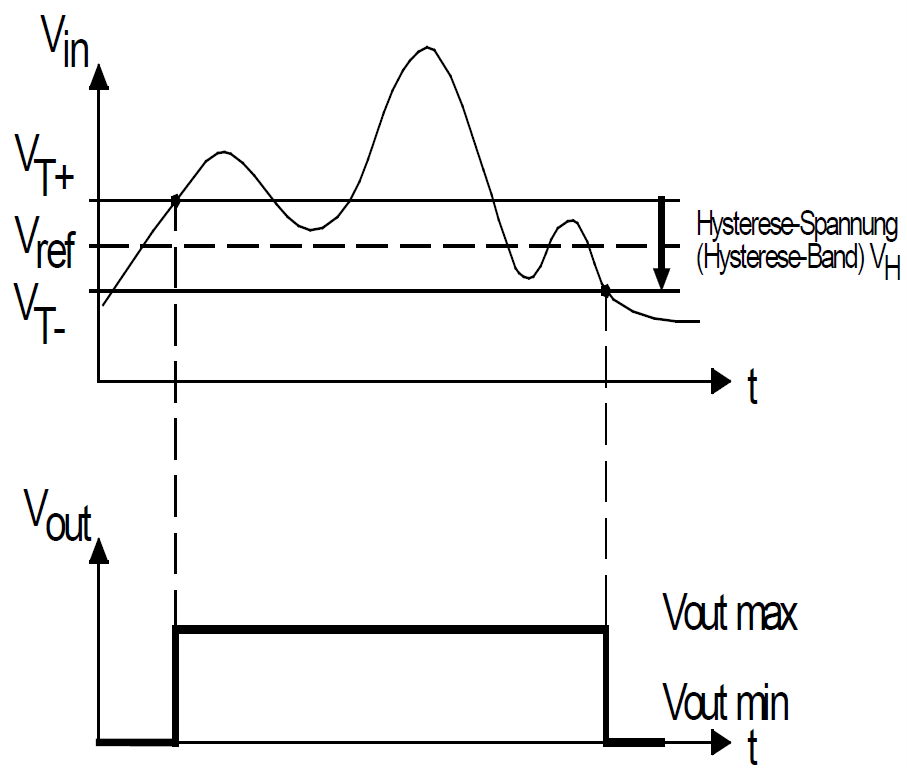
\includegraphics[width=\columnwidth]{images/signalverlauf_schmitt-trigger.png}
\end{minipage}
\hfill
\begin{minipage}[c]{0.62\columnwidth}
	\textbf{Mitkopplung} auf opp \textrightarrow\ 2 Schaltschwellen, die Hysterese unterdrückt Glitches \\[4pt]
	$V_{T+}$ = \textbf{obere}, $V_{T-}$ = \textbf{untere} Schwelle
	$$ V_H = V_{T+} - V_{T-} > 0 $$
	Die aktive Schwelle hängt vom aktuellen Ausgang ab (inv.: Ausgang high \textrightarrow\ $V_{T+}$ aktiv)
\end{minipage}

\begin{rezept}{Rezept: Schaltschwellen (jede Variante)}
	\begin{steps}
		\item Wo hängt $V_{\rm in}$? \; an opn \textrightarrow\ invertierend, \; an opp \textrightarrow\ nicht-invertierend
		\item $V_{\rm opp}$ per Superposition \textbf{aller} Quellen ($V_{\rm ref}$, $V_{\rm DD}$, GND, $V_{\rm out}$) aufstellen
		\item $V_{\rm out} = V_{\rm out,max}$ einsetzen \textrightarrow\ eine Schwelle; \; $V_{\rm out} = V_{\rm out,min}$ \textrightarrow\ die andere
		\item Inv.: Schwelle $= V_{\rm opp}$; \; nicht-inv.: $V_{\rm opp} = V_{\rm opn}$ ($=V_{\rm ref}$) nach $V_{\rm in}$ auflösen
	\end{steps}
	$$ V_H = (V_{\rm out,max} - V_{\rm out,min})\cdot k_{\rm out} \qquad k_{\rm out} = \text{Teilerfaktor von } V_{\rm out} \text{ nach opp} $$
\end{rezept}

{\renewcommand{\arraystretch}{1.6}
\begin{tabularx}{\columnwidth}{@{}p{0.25\columnwidth} X@{}}
	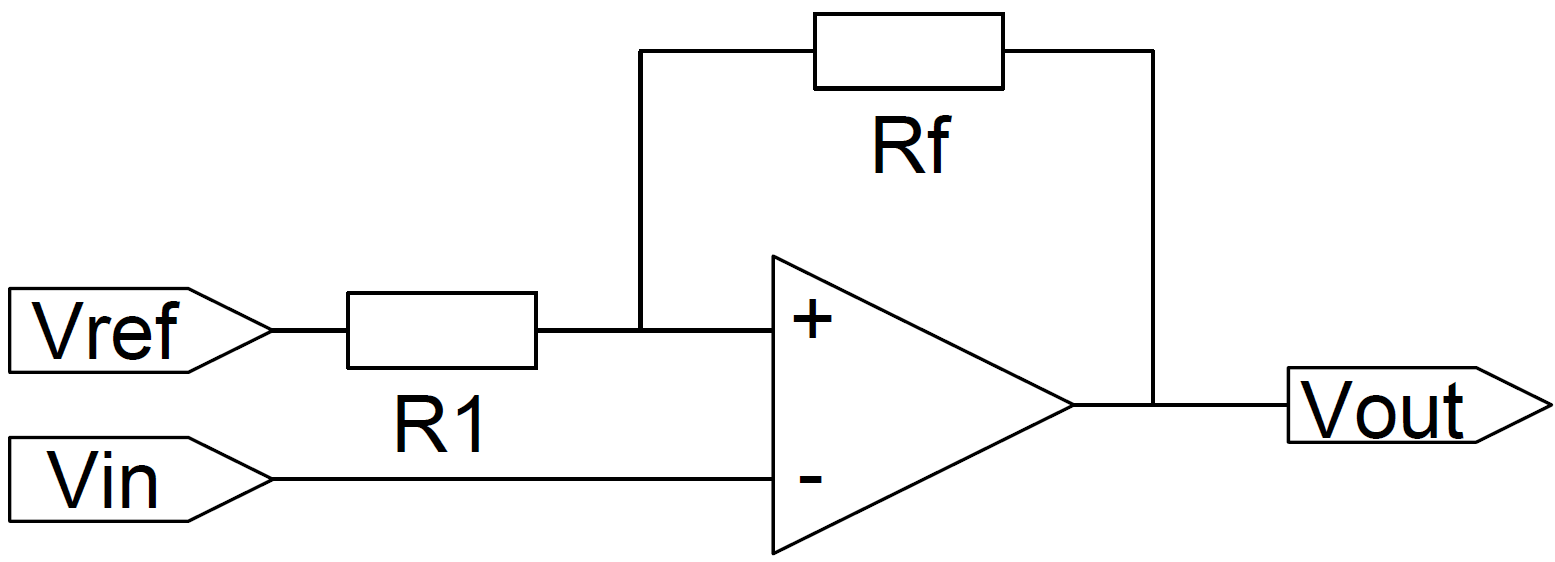
\includegraphics[width=\linewidth,align=c]{images/invertierender_schmitt-trigger.png} &
	\textbf{Invertierend} ($V_{\rm in}$ an opn) \quad Nachteil: Kick-Back auf den Eingang \newline
	$V_{T\pm} = V_{\rm ref}\dfrac{R_f}{R_1+R_f} + V_{\rm out,max/min}\dfrac{R_1}{R_1+R_f}$ \newline
	$V_H = (V_{\rm out,max}-V_{\rm out,min})\dfrac{R_1}{R_1+R_f}$ \\
	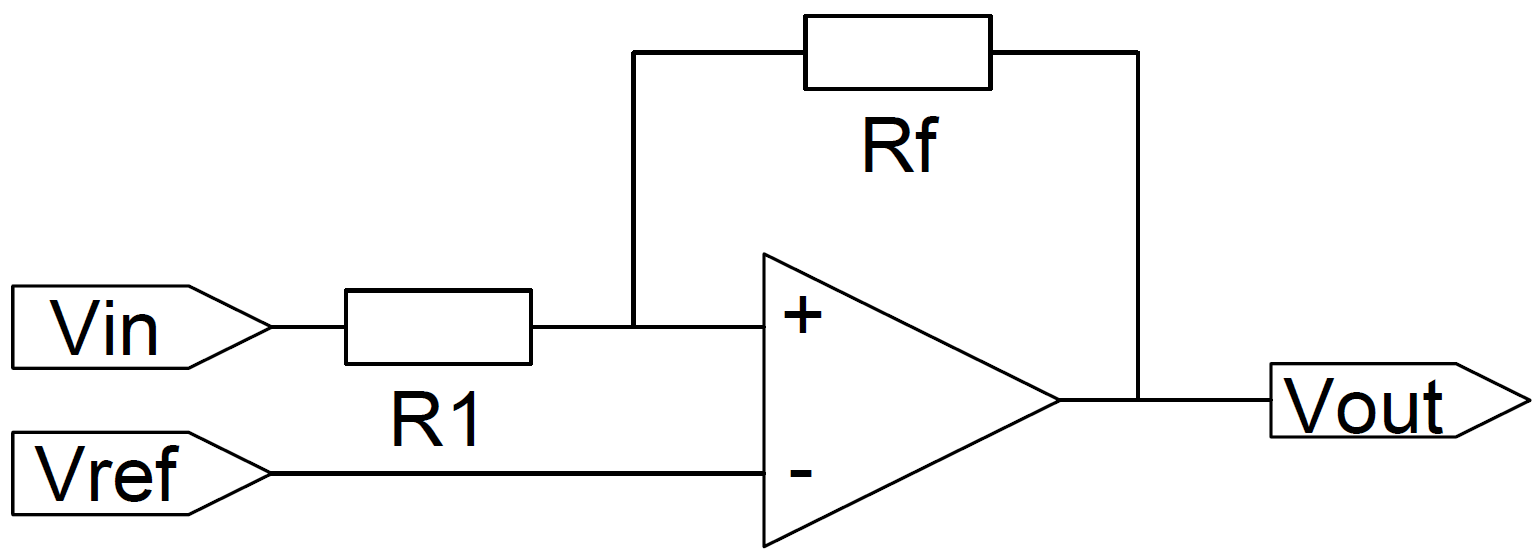
\includegraphics[width=\linewidth,align=c]{images/nichtinvertierender_schmitt-trigger.png} &
	\textbf{Nicht-invertierend} ($V_{\rm in}$ über $R_1$ an opp) \newline
	$V_{T\pm} = V_{\rm ref}\dfrac{R_1+R_f}{R_f} - V_{\rm out,min/max}\dfrac{R_1}{R_f}$ \newline
	$V_H = (V_{\rm out,max}-V_{\rm out,min})\dfrac{R_1}{R_f}$ \\
	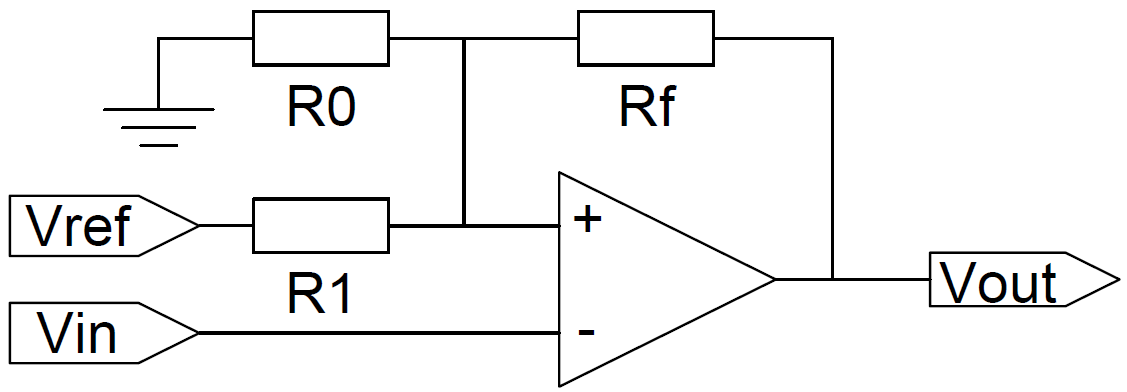
\includegraphics[width=\linewidth,align=c]{images/inv_schmitt-trigger_schaltschwellen.png} &
	\textbf{Frei wählbare Schwellen} (inv., $R_0$ nach GND oder $V_{\rm DD}$) \newline
	$V_{\rm opp} = V_{\rm ref}\dfrac{R_f\parallel R_0}{R_1 + R_f\parallel R_0} + V_{\rm out}\dfrac{R_1\parallel R_0}{R_1\parallel R_0 + R_f}$ \newline
	2 Gleichungen ($V_{T+}$, $V_{T-}$), 3 Unbekannte \textrightarrow\ ein $R$ frei wählen
\end{tabularx}}

\begin{warnbox}
	\small
	\warn{\textit{$V_{\rm os}$, invertente ($V_{\rm in}$ su opn): entrambe le soglie $+V_{\rm os}$.}}
	\warn{\textit{$V_{\rm os}$, non invertente: soglie spostate di $-V_{\rm os}\frac{R_1+R_f}{R_f}$.}}
	\warn{\textit{$V_{\rm out,max/min}$ = valori veri dell'uscita: se non è rail-to-rail l'escursione è minore e l'isteresi pure.}}
	\warn{\textit{Soglie e isteresi non regolabili in modo indipendente (inv. e non inv.) \textrightarrow\ variante con $R_0$.}}
\end{warnbox}

\subsection{Oszillatoren}\label{sec:oszillator}

\subsubsection*{A) Integrator + Schmitt-Trigger \textrightarrow\ Dreieck / Rechteck}

\begin{minipage}[c]{0.4\columnwidth}
	\centering
	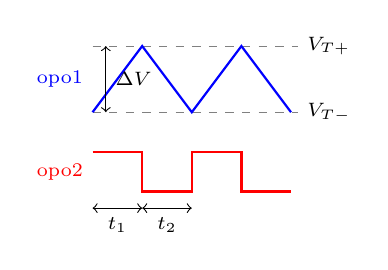
\begin{tikzpicture}[x=0.42cm,y=0.42cm,font=\scriptsize]
		\draw[gray,dashed] (0,1)--(6.2,1) node[right,black]{$V_{T+}$};
		\draw[gray,dashed] (0,-1)--(6.2,-1) node[right,black]{$V_{T-}$};
		\draw[blue,thick] (0,-1)--(1.5,1)--(3,-1)--(4.5,1)--(6,-1);
		\node[blue,left] at (0,0) {opo1};
		\draw[<->] (0.4,-1)--(0.4,1) node[midway,right]{$\Delta V$};
		\draw[red,thick] (0,-2.2)--(1.5,-2.2)--(1.5,-3.4)--(3,-3.4)--(3,-2.2)--(4.5,-2.2)--(4.5,-3.4)--(6,-3.4);
		\node[red,left] at (0,-2.8) {opo2};
		\draw[<->] (0,-3.9)--(1.5,-3.9) node[midway,below]{$t_1$};
		\draw[<->] (1.5,-3.9)--(3,-3.9) node[midway,below]{$t_2$};
	\end{tikzpicture}
\end{minipage}
\hfill
\begin{minipage}[c]{0.58\columnwidth}
	\begin{rezept}{Rezept: Frequenz}
		\begin{steps}
			\item Schwellen $V_{T\pm}$ (\ref{sec:schmitt}) \textrightarrow\ $\Delta V = V_{T+}-V_{T-}$
			\item Strom pro Zustand: $I = \dfrac{V_{\rm Quelle}-V_{\rm COM}}{R}$
			\item Rampenzeit: $t = \dfrac{C\,\Delta V}{|I|}$ \; (linear, Kap.~\ref{sec:opamp-C})
			\item $T = t_1 + t_2$, \; $f=\dfrac1T$; \; symm.: $f = \dfrac{|I|}{2C\,\Delta V}$
		\end{steps}
	\end{rezept}
\end{minipage}

\vspace{4pt}
Gemessen meist tiefer als berechnet: Toleranz von $C$ und Verzögerung des Komparators. \\[2pt]
\textbf{VCO}: $I \propto V_{\rm in}$ \textrightarrow\ $f \propto V_{\rm in}$; \; ungleiche Ströme \textrightarrow\ Duty-Cycle $\neq 50\,\%$
\warn{\textit{Se VDD e VCOM raddoppiano, raddoppiano sia $\Delta V$ sia $I$: f non cambia.}}

\subsubsection*{B) RC-Relaxationsoszillator (Schmitt-Trigger + RC)}

\begin{minipage}[c]{0.4\columnwidth}
	\centering
	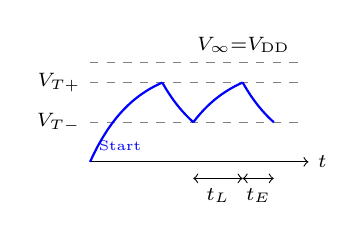
\begin{tikzpicture}[x=0.38cm,y=0.42cm,font=\scriptsize]
		\draw[->] (0,0)--(7.3,0) node[right]{$t$};
		\draw[gray,dashed] (0,3)--(7,3) node[above left,black]{$V_\infty{=}V_{\rm DD}$};
		\draw[gray,dashed] (0,2.4)--(7,2.4);
		\draw[gray,dashed] (0,1.2)--(7,1.2);
		\node[left] at (0,2.4) {$V_{T+}$};
		\node[left] at (0,1.2) {$V_{T-}$};
		\draw[blue,thick,domain=0:1.609,samples=20] plot ({1.5*\x},{3-3*exp(-\x)});
		\draw[blue,thick,domain=0:0.693,samples=15] plot ({1.5*(1.609+\x)},{2.4*exp(-\x)});
		\draw[blue,thick,domain=0:1.099,samples=20] plot ({1.5*(2.302+\x)},{3-1.8*exp(-\x)});
		\draw[blue,thick,domain=0:0.693,samples=15] plot ({1.5*(3.401+\x)},{2.4*exp(-\x)});
		\node[blue,font=\tiny] at (1.0,0.5) {Start};
		\draw[<->] (3.45,-0.5)--(5.1,-0.5) node[midway,below]{$t_L$};
		\draw[<->] (5.1,-0.5)--(6.14,-0.5) node[midway,below]{$t_E$};
	\end{tikzpicture}
\end{minipage}
\hfill
\begin{minipage}[c]{0.58\columnwidth}
	$$ V_C(t) = V_\infty + (V_{\rm start}-V_\infty)\,\e^{-t/RC} $$
	$$ \boxed{ t = RC\,\ln\frac{V_\infty - V_{\rm start}}{V_\infty - V_{\rm end}} } $$
	Laden ($V_\infty = V_{\rm DD}$): $V_{T-}\to V_{T+}$ \\
	Entladen ($V_\infty = 0$): $V_{T+}\to V_{T-}$ \\
	$T = t_L + t_E$
\end{minipage}

\vspace{4pt}
\warn{\textit{Il primo semiperiodo parte da 0 V (o dal valore dato), non da $V_{T-}$: dura di più.}}
\warn{\textit{RC $\Rightarrow$ esponenziale, serve il ln; integratore $\Rightarrow$ rampa lineare.}}
